\documentclass[twoside=true, openright, pdftex, bibliography=totoc, chapterprefix=true, appendixprefix=true, numbers=noenddot, parskip=half, titlepage, index=totoc, headlines=3, footlines=2, headings=normal, language=german]{scrartcl}
\usepackage{xcolor}
\usepackage[utf8]{inputenc}                   % latin9 utf8
\usepackage[german]{babel}                    % german, ngerman, english
\bibliographystyle{unsrt}
\usepackage{booktabs}
\usepackage{subfig}
\usepackage{amsmath,amssymb}
\usepackage{graphicx}
\usepackage[colorlinks=true,citecolor=black,linkcolor=black,urlcolor=blue]{hyperref}
\usepackage{tikz,graphics,color,fullpage,float,caption}
\usepackage{cleveref}[german]
%\bibliographystyle{ieeetran}
%\bibliographystyle{ieeetr}
%\bibliographystyle{plain}
%\hypersetup{colorlinks=false}
%\hypersetup{colorlinks=true,urlcolor=black,linkcolor=black}
%single spacing is default
%\onehalfspacing
%\singlespacing
%\setlength{\footskip}{1cm}

\author{Marcel Rothering}
\title{Performance-Metriken und Evaluation von Supervised Machine Learning Algorithmen}


\begin{document}
\maketitle
% Um eine noch besseren Schätzwert für die Performance ungesehener Daten zu erzielen, kann man K-Fold Cross-Validation verwenden.
\section{Einführung}
Die Daten wurden aufbereitet, neue Features abgeleitet und verschieden Machine Learning Modelle trainiert. Doch wie bewertet man die Performance dieser Modelle? Wie entscheide ich mich z.B. zwischen einem Neuronalen Netz, Random Forest oder Gradient Boosting Classifier? Hierfür verwendet man im Machine Learning Bereich sogenannte Performance Metriken. Diese werden für einen Testdatensatz (\textit{Hold-out Set}) evaluiert, welches nicht zum Training des Modells verwendet wurde, um die Performance für ungesehene Daten abzuschätzen. Doch welche Metriken werden für welches Problem eigentlich verwendet und wann ist die Performance ausreichend?

In diesem Blogbeitrag werden wir verschiedene Performance Metriken für Supervised Machine Learning vorstellen. Zunächst starten wir mit den Metriken für Klassifikation, gefolgt von denen für Regressionsmodelle. Anschließend stellen wir kurz das Kreuzvalidierungsverfahren vor, um einen noch besseren Schätzwert für die Performance eines Modells auf ungesehene Daten zu ermitteln. 

\section{Metriken für Klassifaktionsmodelle}
Klassifikationsmodelle könne in verschiedene Kategorien eingeteilt werden: Binäre, Multi-class, multi-label und hierarchische Klassifikation. Die meisten Performance Metriken für die verschiedenen Kategorien lassen sich aus denen der binären Klassifikation ableiten, weshalb wir uns in diesem Blogbeitrag auf binäre Klassifikation fokussieren. Der interessierte Leser findet die Ableitungen der Performance-Metriken auf komplexere Klassifikationsmodelle in \cite{Sokolova:2009:SAP:1542545.1542682}.

\paragraph{Accuracy}
Die wohl einfachste Performance Metrik für Klassifikationsmodelle ist die Accuarcy/Genauigkeit. Diese lässt sich wie folgt berechnen
\begin{equation}
\mathrm{Acc} = \frac{\# correct\ predictions }{\# all\ predictions}.
\end{equation}
Hat man z.B. 55 richtige Vorhersagen für 100 Beobachtungen gemacht, dann ist die Genauigkeit 55~\% und nicht viel besser als der Zufall \footnote{Das gilt nur, falls es sich hier um zwei ausbalanzierte Klassen handelt.}. Letztere Aussage gilt nur, falls die beiden Klassen, 0 und 1, ausbalanziert sind, d.h. im Datensatz gibt es ungefähr gleich viele Beobachten der Klasse 0 und der Klasse 1. Falls eine der beiden Klassen unter- oder überrepresentiert ist, dann ist die Accuarcy keine gute Metrik. Stellen Sie sich zum Beispiel eine Datensatz vor in dem 95 Beobachtungen zur Klasse 0 gehören und nur 5 zur Klasse 1. Ein Modell, welches nun immer die Klasse 0 vorhersagen würde erzielt dann eine Accuracy von 95~\%. Klingt gut, ist in diesem Fall aber schlecht und die Accuracy ist hier nicht geignet. Bei solch einem Problem ist es von Vorteil die Klassifikationsergebnisse in eine sogenannte Confusion-Matrix aufzuteilen.

\paragraph{Confusion-Matrix}

\begin{table}%
  \centering
  \subfloat[][Confusion-Matrix.\label{conf}]{
\centering
%\caption{Confusion Matrix als Performance Metrik für ein Binäres Klassifikationsproblem.}
\label{my-label}
\begin{tabular}{@{}ccc@{}}
\toprule
\multicolumn{1}{l}{}                                 & \begin{tabular}[c]{@{}c@{}}Predicted:\\ 0\end{tabular} & \begin{tabular}[c]{@{}c@{}}Predicted:\\ 1\end{tabular} \\ \midrule
\begin{tabular}[c]{@{}c@{}}Actual: \\ 0\end{tabular} & TN                                                     & FP                                                     \\
\begin{tabular}[c]{@{}c@{}}Actual:\\ 1\end{tabular}  & FN                                                     & TP                                                    
\end{tabular}
%\end{table}
}
  \qquad
  \subfloat[][Normierte Confusion-Matrix.\label{confNorm}]{
%\caption{Confusion Matrix als Performance Metrik für ein Binäres Klassifikationsproblem.}
%\label{my-label}
\begin{tabular}{@{}ccc@{}}
\toprule
\multicolumn{1}{l}{}                                 & \begin{tabular}[c]{@{}c@{}}Predicted:\\ 0\end{tabular} & \begin{tabular}[c]{@{}c@{}}Predicted:\\ 1\end{tabular} \\ \midrule
\begin{tabular}[c]{@{}c@{}}Actual: \\ 0\end{tabular} & $\frac{\mathrm{TN}}{\# all\ negatives}$                                                     & $\frac{\mathrm{FP}}{\# all\ negatives}$                                                     \\
\begin{tabular}[c]{@{}c@{}}Actual:\\ 1\end{tabular}  & $\frac{\mathrm{FN}}{\# all\ positives}$                                                     & $\frac{\mathrm{TP}}{\# all\ positives}$                                                    
\end{tabular}
}
  \caption{Tabellarische Darstellung der Confusion Matrix (links) und der normierten Confusion-Matrix (rechts)}%
  \label{tbl:table}%
\end{table}



In Tabelle \ref{conf} ist die allgemeine Confusion-Matrix gezeigt. Diese beinhaltet als Elemente die Anzahl an korrekten positiven (TP), korrekten negativen (TN), an falschen positiven (FP) und falschen negativen Vorhersagen. Den beiden Klassen werden hierbei die beiden Attribute positiv für Klasse 1 und negativ für Klasse 0 zugeordnet. Oftmals wird die Confusion Matrix noch normiert (siehe Tabelle \ref{confNorm}), da es schwierig ist anhand der absoluten Zahlen die Performance einzuschätzen. Die Elemente spiegeln dann die Raten TNR, FPR, FNR und TPR wider. Ein Zahlenbeispiel ist in den Tabellen \ref{ZahlenBeispiel} aufgeführt. Dort können wir direkt ablesen, dass 21~\% der Vorhersagen für die negative Klasse falsch sind und 23~\% der Vorhersagen für die positive Klasse. Diese beiden Fehler werden oft auch als Type 2 und Type 1 Fehlerraten bezeichnet.  Welchen Fehler man nun reduzieren möchte hängt stark vom Anwendungsfall des Modells ab. Soll dieses Modell beispielsweise als Spam Filter dienen (Spam ist hier die positive Klasse), so würde man gerne die Rate der als falsch positiv klassifizierten E-Mails reduzieren (geringe FNR). Denn es ist weitaus dramatischer, wenn eine wichtige Mail mal im Spamordner landet, als das eine Spam E-Mail einmal nicht als solche erkannt wurde (höhere FPR). Umgekehrte Bedürfnisse stellen wir zum Beispiel an ein Modell welches jugendfreie Filme (Klasse 1) herausfiltern soll. Lieber lassen wir unsere Kinder weniger Filme anschauen (höhere FNR), als das nicht jugendfreie Filme freigegeben werden (geringe FPR).


\begin{table}%
  \centering
  \subfloat[][Confusion-Matrix.]{
\centering
%\caption{Confusion Matrix als Performance Metrik für ein Binäres Klassifikationsproblem.}
\label{my-label}
\begin{tabular}{@{}ccc@{}}
\toprule
\multicolumn{1}{l}{}                                 & \begin{tabular}[c]{@{}c@{}}Predicted:\\ 0\end{tabular} & \begin{tabular}[c]{@{}c@{}}Predicted:\\ 1\end{tabular} \\ \midrule
\begin{tabular}[c]{@{}c@{}}Actual: \\ 0\end{tabular} & 83 & 22 \\
\begin{tabular}[c]{@{}c@{}}Actual:\\ 1\end{tabular}  & 17  & 57
\end{tabular}
%\end{table}
}
  \qquad
  \subfloat[][Normierte Confusion-Matrix]{
%\caption{Confusion Matrix als Performance Metrik für ein Binäres Klassifikationsproblem.}
%\label{my-label}
\begin{tabular}{@{}ccc@{}}
\toprule
\multicolumn{1}{l}{}                                 & \begin{tabular}[c]{@{}c@{}}Predicted:\\ 0\end{tabular} & \begin{tabular}[c]{@{}c@{}}Predicted:\\ 1\end{tabular} \\ \midrule
\begin{tabular}[c]{@{}c@{}}Actual: \\ 0\end{tabular} &0.79& 0.21 \\
\begin{tabular}[c]{@{}c@{}}Actual:\\ 1\end{tabular}  & 0.23 & 0.77 
\end{tabular}
}
  \caption{Zahlenbeispiel für die Confusion Matrix (links) und für die normierten Confusion-Matrix (rechts) \label{ZahlenBeispiel}}%
  \label{tbl:table}%
\end{table}

Viele weitere Metriken lassen sich aus der Confusion Matrix berechnen. Weit verbreitete Metriken sind hier die Precison, der Recall und der F1-Score, welche im folgenden kurz besprochen werden.

\paragraph{Precison, Recall und F1-Score}

\begin{eqnarray}
  \mathrm{Precision} &=& \frac{TP}{TP + FP} = \frac{TP}{P^*} \\
  \mathrm{Recall} &=& \frac{TP}{TP + FN} = \frac{TP}{P}\\
  F1 &=& \left(\frac{1/Precison + 1/Recall}{2}\right)^{-1}
\end{eqnarray}


\begin{figure*}[t!]
  \centering
        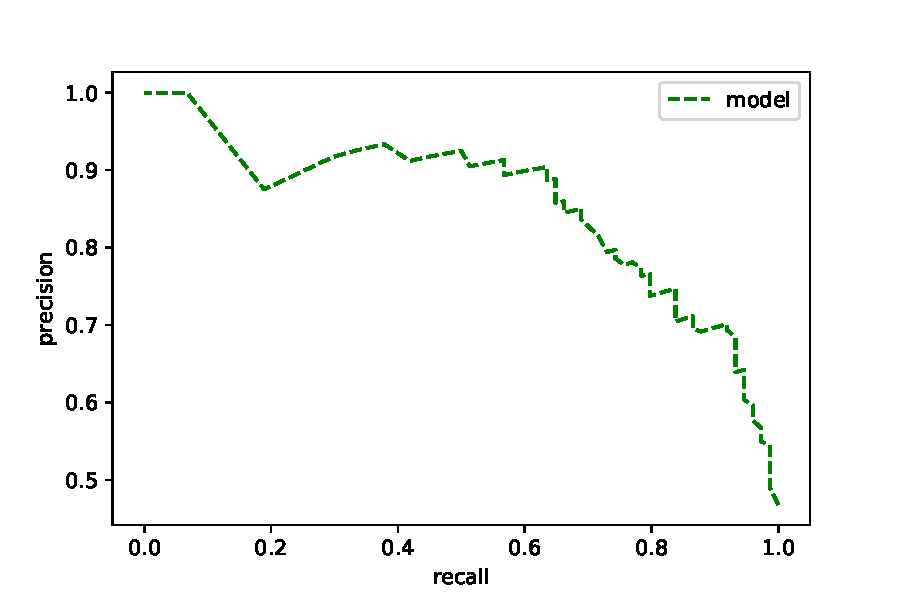
\includegraphics[width=.45\textwidth]{precRecall.pdf}\
        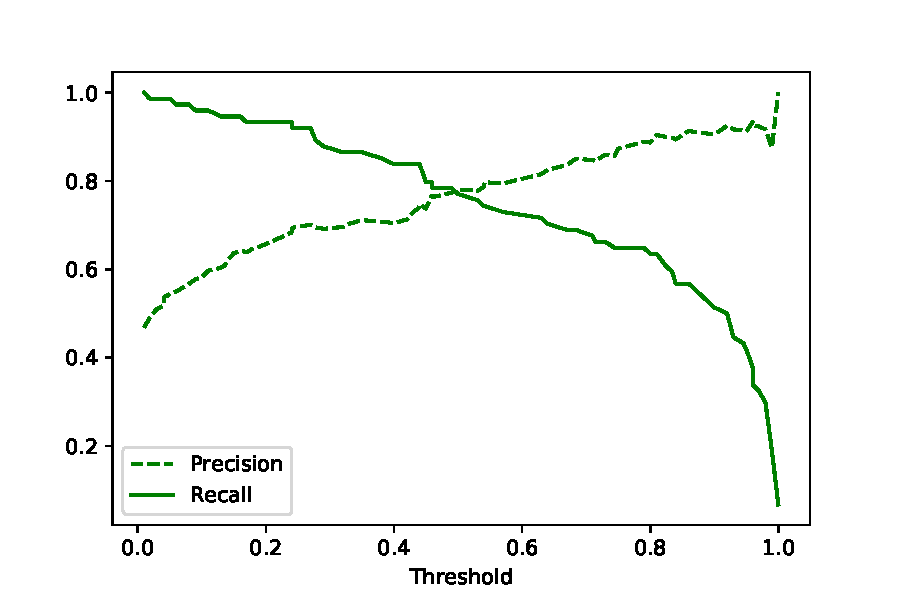
\includegraphics[width=.45\textwidth]{precRecallVsThreshold.pdf}
    \caption{Precision-Recall Kurve (links) eines binären Klassifikationsmodells und Werte für Precision (Recall) für verschiedene Thresholds/Schwellwerte des Klassifikationsmodells (rechts). \label{preRec}}
\end{figure*}

\paragraph{Receiver Opeator Charateristic}

\begin{figure*}[t!]
  \centering
        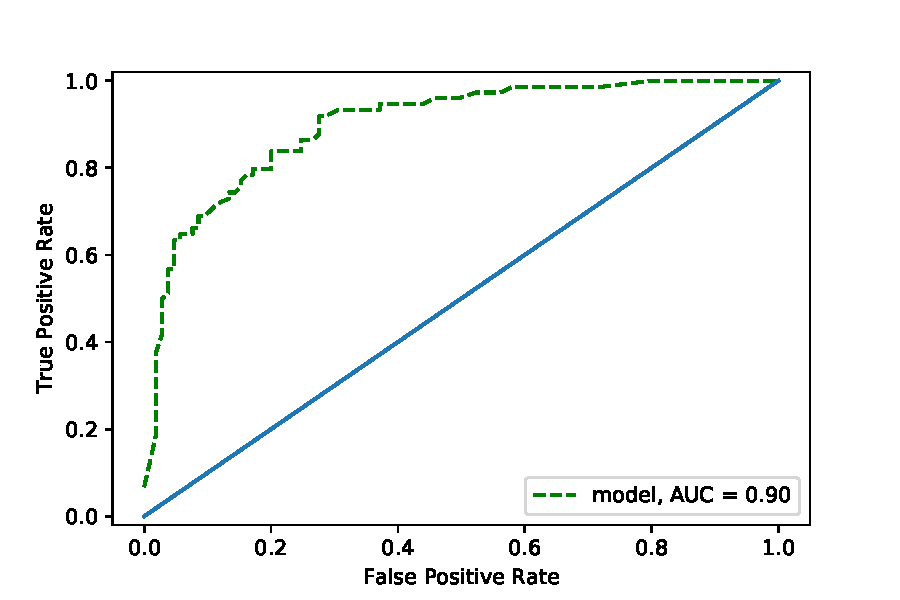
\includegraphics[width=.45\textwidth]{roc.pdf}
    \caption{ROC Kurve für ein Klassifikationsmodell (grün) und für eine zufällige Klassifikation (blau). \label{roc}}
\end{figure*}

Viele mehr wie sensitivity, hamming loss, etc.

Manche dieser Metriken wie Precision, Recall und F1 sind außerdem invariant unter einer bestimmten Veränderung der Confusion Matrix. Verändert man beispielsweise die Anzahl der True Negatives (TNs), so hat dies keine Auswirkung auf diese Performance Metriken. Dem sollte man sich bewusst sein, wenn man beispielsweise auch die Güte der negativen Klasse messen/beschreiben will. Die ROC Kurve hingegen beinhaltet alle Elemente der Confusion Matrix und ist daher nicht invariant unter Veränderung eines einzelnen Elements (nur FPR = FP / (TN + FP) und TPR = TP / (TP + FN).

\section{Metriken für Regressionsmodelle}
\begin{figure*}[t!]
  \centering
        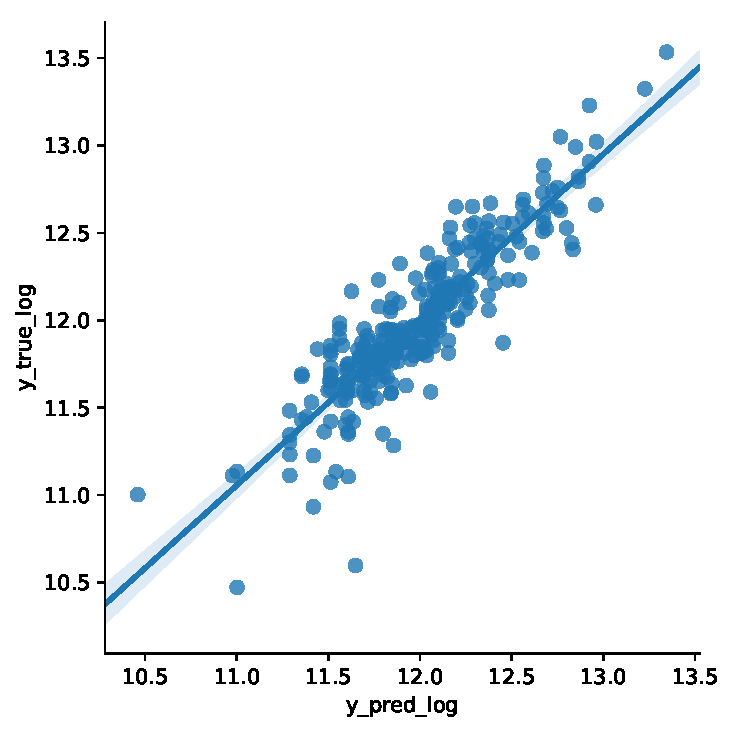
\includegraphics[width=.4\textwidth]{r2.pdf}\
        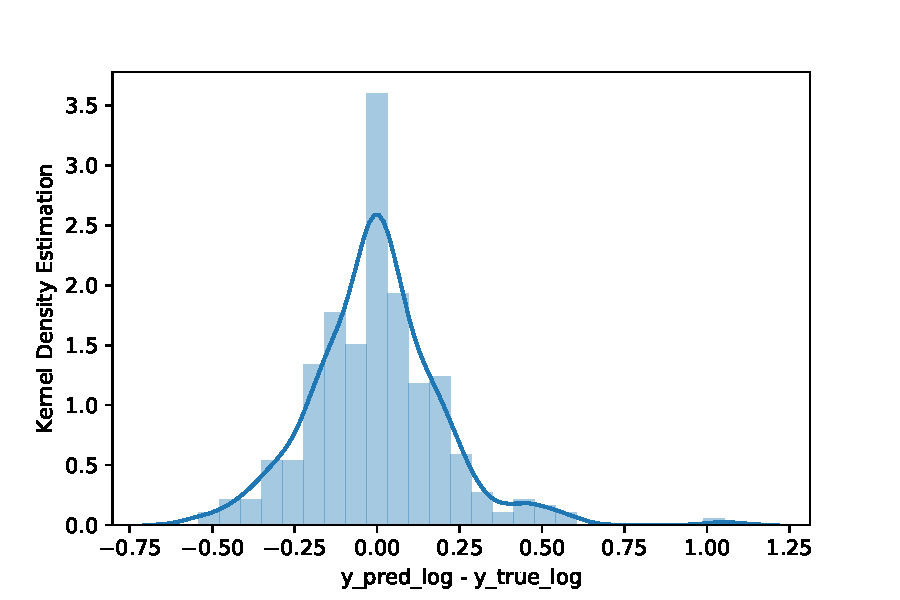
\includegraphics[width=.45\textwidth]{residuen.pdf}
    \caption{Precision-Recall Kurve (links) eines binären Klassifikationsmodells und Werte für Precision (Recall) für verschiedene Thresholds/Schwellwerte des Klassifikationsmodells (rechts). \label{preRec}}
  \end{figure*}

  Bic, AIC, analysis of Variance (Anova, etc.)
\section{K-Fold Kreuzvalidierung}
In der Regel verwendet man K Fold Cross Validation für Modelle, welche nicht all zu lang für das Training brauchen, wie z.B. CNNs. Außerdem ausgenommen sind Forecasting Modelle für Zeitreihenanalyse, wie ARIMA, etc.

\bibliography{literatur.bib} 

\end{document}
%% end of file
